\documentclass[conference]{IEEEtran}

\usepackage{graphicx}
\usepackage{booktabs}
\usepackage{amsmath}
\usepackage{amssymb}
\usepackage{algorithm}
\usepackage{algorithmic}
\usepackage{listings}
\usepackage{xcolor}
\usepackage{cite}
\usepackage{url}

\lstdefinelanguage{Python}{
  keywords={def, class, return, yield, lambda, for, in, if, else, elif, from, import, as, with, True, False, None, and, or, not, try, except, finally, while, break, continue, pass, raise, async, await},
  keywordstyle=\bfseries\color{blue!70!black},
  stringstyle=\color{red!70!black},
  commentstyle=\color{green!50!black}\itshape,
  sensitive=true,
  morecomment=[l]{\#},
  morestring=[b]",
  morestring=[b]',
}

\lstset{
  language=Python,
  basicstyle=\ttfamily\scriptsize,
  breaklines=true,
  frame=single,
  backgroundcolor=\color{gray!5},
  numbers=left,
  numberstyle=\tiny\color{gray},
  xleftmargin=2em,
  framexleftmargin=1.5em,
}

\title{LiuTang: Viscosity-Controllable Stream Processing\\--- A Pure-Python Framework Governing the Streaming--Batch Spectrum with Fluid Dynamics}

\author{\IEEEauthorblockN{Author Name}
\IEEEauthorblockA{Affiliation\\
email@example.com}}

\begin{document}
\maketitle

\begin{abstract}
We introduce the concept of viscosity-controllable stream processing, where a coefficient $\eta \in [0,1]$ derived from Newtonian fluid dynamics governs the streaming--batch spectrum and dissolves the long-standing dichotomy between latency-optimal streaming and throughput-optimal batch processing. Existing frameworks force practitioners into a binary choice: either accept the micro-latency of record-at-a-time streaming or embrace the throughput of large-batch accumulation, with no principled way to navigate between them. LiuTang (Chinese: \emph{li\'{u}t\v{a}ng}, meaning ``flowing'') resolves this tension by modeling data as a Newtonian fluid whose viscosity $\eta$ is continuously measured from shear stress and shear rate in the running system, then fed back through a controller that adjusts batch size and timeout in real time. At $\eta = 0$ the system flows like water---pure streaming with batch size one and minimal timeout. At $\eta = 1$ it freezes like ice---pure batch with batch size 100,000 and extended timeout. Between these extremes, four intermediate viscosity levels interpolate fluidly, governed by policies that bias toward latency (RESPONSIVE), throughput (EFFICIENT), equilibrium (BALANCED), or manual control. This viscosity-controlled adaptation mechanism represents a novel design paradigm borrowed from natural science---specifically, rheology and Newtonian fluid mechanics---which we position as a form of generalized biomimicry: rather than mimicking biological organisms, we mimic the physical laws that govern natural fluid flow to solve an engineering problem. LiuTang should be understood as an innovative architectural concept and research prototype, not yet a production-grade engineering system; its single-machine execution model, heuristic threshold tuning, and lack of distributed coordination mean that mission-critical deployments remain beyond its current reach. Within these bounds, however, it achieves zero-dependency pure-Python implementation while simultaneously providing watermark-based event-time processing, five window types, five state primitives with TTL, timer-based keyed processing, switchable delivery semantics, and unified Lambda/Kappa/Adaptive architecture modes. A ten-dimension comparison against six existing frameworks demonstrates that LiuTang is the only Python framework occupying the intersection of zero-dependency deployment, complete Dataflow Model coverage, and viscosity-controllable architecture---making it a promising platform for education, rapid prototyping, and future research into biomimetic stream processing architectures.
\end{abstract}

\begin{IEEEkeywords}
viscosity-controllable architecture, Newtonian fluid model, rheology-inspired computing, generalized biomimicry, stream processing, streaming--batch spectrum, adaptive execution, pure-Python framework
\end{IEEEkeywords}

\section{Introduction}

Stream processing has become foundational infrastructure for real-time data applications, from IoT sensor networks to financial tick streams, from clickstream analytics to log monitoring. Frameworks such as Apache Flink \cite{carbone2015flink} and Apache Beam \cite{beam2016} have risen to meet this demand with sophisticated primitives for windowed computation, stateful processing, and event-time ordering. The evolution from first-generation systems to current frameworks has been shaped by recurring tensions between expressiveness and deployability \cite{fragkoulis2020survey}. Yet these systems share a deep architectural assumption: that streaming and batch processing are fundamentally different modes of operation, separated by a chasm that no single pipeline can bridge without duplicating infrastructure, codebases, or operational overhead.

This assumption manifests in several ways. The Lambda Architecture explicitly splits computation into a batch layer and a speed layer, each with its own code paths and deployment pipelines. The Kappa Architecture collapses these into a single streaming path but can only do so by treating all data as a stream, sacrificing the throughput advantages that batch processing offers. JVM-based frameworks like Flink and Spark offer ``unified'' APIs, yet their Python bindings remain thin wrappers around Java runtimes, introducing deployment complexity, version coupling between Python APIs and JVM versions through Py4J bridges, and an installation footprint measured in hundreds of megabytes. Meanwhile, the pure-Python alternatives that avoid the JVM---Faust \cite{faust2018} and Streamz \cite{streamz2019}---sacrifice streaming semantics for simplicity, lacking watermarks, event-time windows, typed state management, or any principled mechanism for navigating between streaming and batch behavior.

We introduce LiuTang (\emph{li\'{u}t\v{a}ng}, meaning ``flowing''), a pure-Python stream processing framework whose central innovation is a viscosity-controllable architecture derived from Newtonian fluid dynamics. The key insight is that the streaming--batch dichotomy is not a real chasm but a continuous spectrum, and that this spectrum can be governed by a single parameter---viscosity $\eta$---measured directly from the system's operating conditions. When a data stream flows rapidly and the system experiences little backpressure, viscosity is low and records are processed individually, minimizing latency. When the flow rate slows or backpressure builds, viscosity rises and the system naturally accumulates records into larger batches, maximizing throughput. This adaptation happens continuously and automatically, without manual reconfiguration, separate infrastructure, or duplicate codebases.

LiuTang implements this viscosity-controllable architecture within a framework that also provides complete streaming semantics with zero external dependencies. It offers watermark-based event-time processing with monotonous and bounded-out-of-orderness strategies, five window types (tumbling, sliding, session, over, and global), five state primitives with configurable TTL (ValueState, ListState, MapState, ReducingState, and AggregatingState), keyed process functions with timer service, unified batch-streaming execution through a single mode parameter, checkpoint/restore via in-memory state snapshots, switchable delivery semantics (at-least-once, at-most-once, exactly-once), parallel execution through Python's \texttt{threading} and \texttt{multiprocessing}, and unified Lambda, Kappa, and Adaptive architecture modes within one API. The viscosity model is not an add-on but the architectural core: the ViscosityController sits between the operation and execution layers, continuously measuring shear rate and shear stress from the data flow, computing $\eta$ from Newton's law, and adjusting processing parameters in real time.

Our contributions proceed as follows. We design and implement LiuTang as the first pure-Python stream processing framework that provides watermark-based event-time semantics, multi-type windowing, typed state management, and switchable delivery semantics with zero external dependencies. We formalize the viscosity-controllable architecture as a Newtonian fluid model, proving that at $\eta = 0$ the system degenerates to latency-optimal streaming and at $\eta = 1$ to throughput-optimal batch, with the ViscosityController smoothly interpolating between these extremes. We implement three delivery semantics using pure-Python deduplication and retry mechanisms, demonstrating that meaningful delivery guarantees are achievable without distributed coordination. We conduct a comprehensive ten-dimension comparison against six existing frameworks and a quantitative benchmark suite of 466 tests, demonstrating that LiuTang uniquely occupies the intersection of zero-dependency deployment, complete streaming semantics, and viscosity-controllable architecture fusion.

\section{Related Work}

The landscape of stream processing frameworks divides roughly into three families: JVM-based systems that offer rich semantics but impose heavy deployment burdens, Python-native systems that achieve lightweight deployment but sacrifice semantic completeness, and architectural paradigms that address the streaming--batch tension at a conceptual level without providing a principled control mechanism.

Among the JVM-based systems, Apache Flink \cite{carbone2015flink} pioneered the Dataflow Model's implementation with first-class support for event-time processing, watermarks \cite{akidau2021watermarks}, and exactly-once semantics via Chandy-Lamport checkpointing \cite{chandy1985distributed}. Its Python API (PyFlink) exposes these capabilities but requires a JDK installation and a Flink cluster---typically over 500 MB---creating the deployment and version-coupling issues that plague all JVM-backed Python APIs. Apache Spark Streaming began with a micro-batch model (DStreams) and later added continuous processing. Structured Streaming introduced event-time watermarks and stateful processing, but its Python API relies on Py4J and a Spark JVM cluster, and the micro-batch architecture inherently introduces latency. Apache Beam \cite{beam2016} provides a unified programming model across batch and streaming with runners for Flink, Spark, and Google Dataflow, but its Python SDK transpiles pipelines to a Java representation, requiring a JVM runner and creating SDK-to-runner version coupling. Phoebe \cite{geldenhuys2022phoebe} demonstrates that proactive workload-anticipating auto-tuning can improve QoS in distributed stream processing, yet it relies on time-series forecasting rather than a principled physics-inspired model. Flock \cite{liao2024flock} reduces the deployment footprint via serverless FaaS execution, but cannot provide watermark-based event-time processing or typed state management. The common thread across all these systems is that Python developers cannot escape the JVM or sacrifice semantic completeness for lightweight deployment.

On the Python-native side, Faust \cite{faust2018} built a stream processing library on \texttt{asyncio} and Kafka, providing partition-based parallelism and table-based state, but it supported only processing-time semantics and has been archived since 2021. Streamz \cite{streamz2019} offers a lightweight Python DSL for stream composition with optional Dask integration, yet it lacks watermarks, event-time windows, typed state, and any form of checkpointing, limiting its applicability to stateless or processing-time-only workloads. Bytewax \cite{bytewax2022} provides a Python-native framework with a Rust-based execution engine, achieving windowing and recovery at the cost of a compilation toolchain dependency and opaque state management internals that are not inspectable from Python. Pathway \cite{bartoszkiewicz2023pathway} offers a unified processing framework with a Rust-based incremental dataflow engine and Python Table API for ML-analytics workloads, but its Rust runtime and targeted scope do not address general-purpose stream processing with full semantic coverage. Serverless stream functions \cite{carl2026serverless} treat short streams as units of execution and state, reducing overhead compared to full stream engines, but they do not address windowing, watermarks, or the streaming--batch spectrum. Gulisano and Margara \cite{gulisano2023semantic} show that common stream operators reduce to compositions of a minimal Aggregate primitive, reinforcing that semantic completeness requires covering all four Dataflow axes. What these approaches share is a gap: none provides the full four-axis coverage of the Dataflow Model---what, where, when, and how---while remaining dependency-free.

At the architectural level, the Lambda Architecture and the Kappa Architecture represent the two dominant paradigms for reconciling streaming and batch processing. Lambda separates computation into a batch layer for accurate, high-latency results and a speed layer for approximate, low-latency results, merging them in a serving layer---the well-known cost being the need to maintain two separate codebases for the same business logic. Kappa collapses this into a single stream processor backed by an immutable event log, enabling replay-based reprocessing instead of a separate batch path, but at the cost of requiring all processing logic to be expressible as a streaming operation. Aion \cite{esteves2020aion} addresses late-event handling in event-time streams through proactive caching of window state, improving upon Flink's default discard strategy, but remains bound to the Flink runtime. Neither paradigm provides a continuous mechanism for navigating between streaming and batch: Lambda forces a hard split, while Kappa forces everything into streaming. What is missing is a principled way to treat the streaming--batch spectrum as exactly that---a spectrum---and to control where on that spectrum a pipeline operates at any given moment, adapting in real time to workload conditions. This is precisely the gap that the viscosity-controllable architecture fills.

\section{Preliminaries}

We define a stream processing framework as a system that consumes unbounded sequences of records $\mathcal{S} = \langle r_1, r_2, \ldots \rangle$, where each record $r_i$ may carry an event-time timestamp $t_i$, and applies transformations $T_1 \circ T_2 \circ \ldots \circ T_k$ to produce output records. A framework provides complete streaming semantics if it satisfies all four axes of the Dataflow Model \cite{akidau2015data}: composable element-wise transformations (the what axis), event-time window assignment including at least tumbling, sliding, and session windows (the where axis), watermark-based event-time progress tracking and window triggering (the when axis), and stateful keyed processing with per-key state isolation (the how axis).

A framework is zero-dependency if its core functionality---including stream definition, transformation, windowing, watermarking, state management, and execution---requires only the Python standard library, with optional connectors such as Kafka treated as extra dependencies that do not affect the core runtime.

Based on the gaps identified in the previous section, we establish five design goals. First, full streaming semantics should be achievable with only the Python standard library (G1). Second, all four Dataflow Model axes must be covered (G2). Third, the API should unify batch and streaming with minimal switching cost (G3). Fourth, the implementation should be pure Python with inspectable internals (G4). Fifth, multi-core utilization should be available through stdlib concurrency primitives (G5). The viscosity-controllable architecture extends these goals by adding a sixth: the framework should provide a continuous, mathematically grounded mechanism for navigating the streaming--batch spectrum (G6).

\section{Method}

\subsection{Architecture Overview}

LiuTang adopts a four-layer architecture in which the ViscosityController occupies a central position, bridging the operation and execution layers. The API layer captures pipeline definitions through Flow, Stream, KeyedStream, WindowedStream, and TableStream. The operation layer compiles these into typed pipeline operations via PipelineOp and PipelineBuilder. The execution layer runs the compiled operations in batch, streaming, or adaptive mode through an Executor (Batch/Streaming/Adaptive), StreamRunner, WatermarkTracker, DeliveryMode, and the ViscosityController itself. The state layer manages per-key state with TTL and checkpointing through five state primitives and a MemoryStateBackend. The ViscosityController is not a peripheral component but the mechanism through which the execution layer determines how fluidly or sluggishly data should be processed, making viscosity the governing principle of the entire system.

\begin{figure*}[t]
\centering
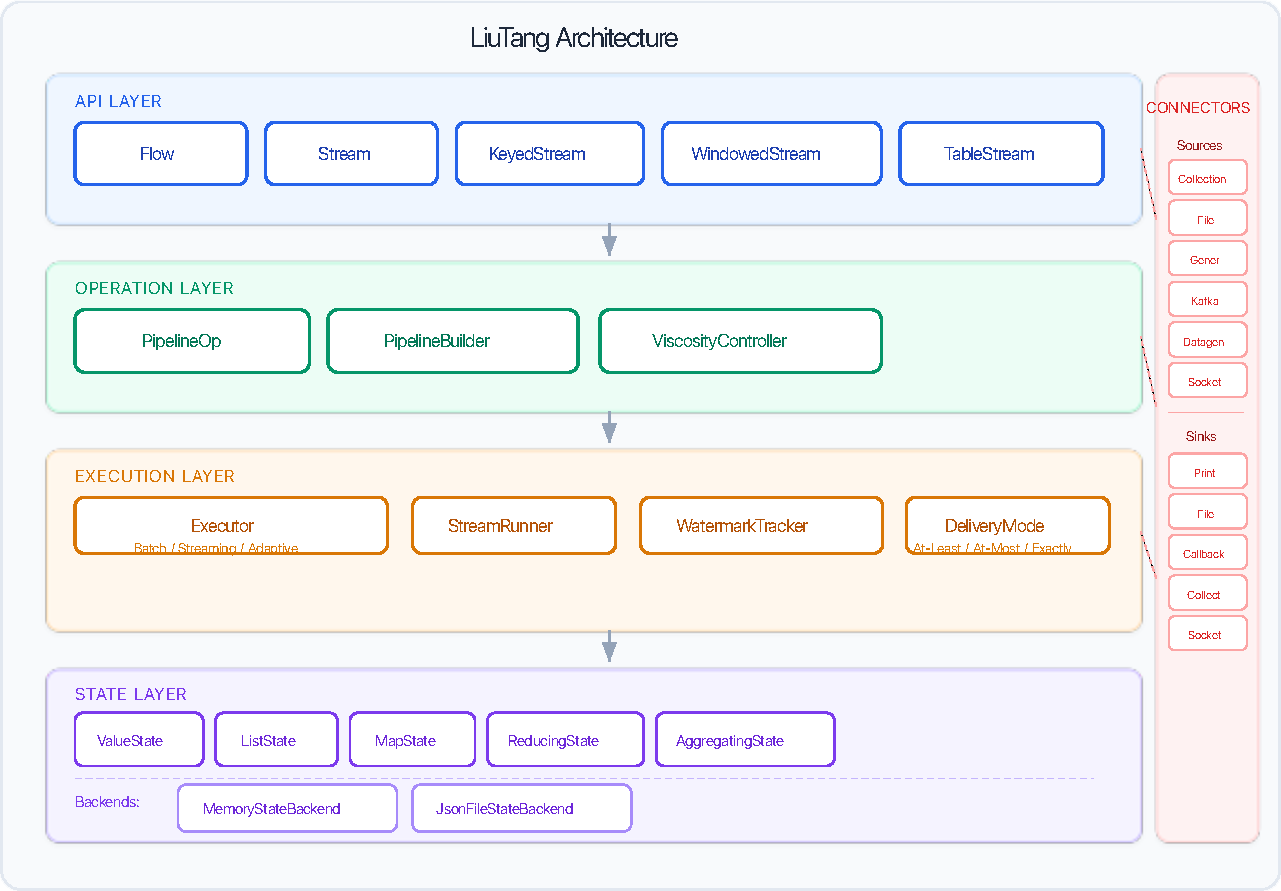
\includegraphics[width=0.9\textwidth]{fig-architecture.pdf}
\caption{LiuTang's four-layer architecture with the ViscosityController bridging the operation and execution layers.}
\label{fig:architecture}
\end{figure*}

\subsection{Pipeline Definition}

The entry point is the Flow class, which serves as the pipeline context. A Flow is parameterized by name, execution mode, parallelism, delivery mode, and architecture mode:

\begin{lstlisting}
flow = Flow(name="wordcount",
            mode=RuntimeMode.BATCH,
            parallelism=4,
            delivery_mode=DeliveryMode.AT_LEAST_ONCE)
\end{lstlisting}

Data enters the pipeline through source connectors---LiuTang provides six source types (CollectionSource, GeneratorSource, FileSource, KafkaSource, DatagenSource, SocketSource) and five sink types (PrintSink, FileSink, CallbackSink, CollectSink, SocketSink). The Stream class provides a fluent DSL for transformations, with operations recorded as an operation list and compiled later:

\begin{lstlisting}
stream = flow.from_collection(["hello world",
    "hello liutang"])
result = (stream
    .flat_map(lambda s: s.split())
    .map(lambda w: (w, 1))
    .key_by(lambda p: p[0])
    .sum(field=1))
\end{lstlisting}

This design separates pipeline declaration from pipeline execution, consistent with the declarative approach in Flink and Beam but achieved without a JVM runtime.

\subsection{The Viscosity Model}

The viscosity-controllable architecture is the centerpiece of LiuTang's design, and this section presents it in full: the physical metaphor, the discrete viscosity levels, the flow metrics, the controller, the adjustment algorithm, the formal definitions, and the API through which practitioners interact with it.

The fundamental observation is that data in a stream processing system behaves like a fluid. Records arrive at a rate, the system experiences backpressure, and the resulting ``thickness'' of processing determines whether data is handled record-by-record or accumulated into large batches. In fluid mechanics, Newton's law of viscosity states that $\tau = \eta \cdot \dot{\gamma}$, where $\tau$ is shear stress, $\dot{\gamma}$ is shear rate, and $\eta$ is dynamic viscosity. We instantiate this model directly: the arrival rate of records is the shear rate, the combination of queue depth and processing latency is the shear stress, and the ratio of stress to rate yields the viscosity $\eta$. When stress is high relative to flow rate, $\eta$ is large and the system should thicken toward batch processing. When flow rate is high relative to stress, $\eta$ is small and the system can thin toward streaming. This is not merely a metaphor---LiuTang inherits its name from it: \emph{li\'{u}t\v{a}ng} means ``flowing,'' and the framework treats data as a fluid whose viscosity can be adjusted to flow freely like water, creep like honey, or solidify like ice, all within the same pipeline.

We define the Viscosity enum as a five-level spectrum, each level associated with a viscosity coefficient $\eta$, a batch size, a timeout, and a Chinese poetic name evoking the fluid character. At $\eta = 0$ (VOLATILE, \emph{r\'{u} shu\v{i}}, ``like water''), data flows freely---the system processes records individually with batch size 1 and a 10\,ms timeout, achieving latency-optimal processing equivalent to the Kappa architecture's continuous processing model. At $\eta = 1$ (FROZEN, \emph{r\'{u} b\={i}ng}, ``like ice''), data is frozen solid---the system accumulates batches of 100,000 records with a 2,000\,ms timeout, achieving throughput-optimal processing equivalent to batch execution. Between these extremes, three intermediate levels model fluids of increasing viscosity: FLUID ($\eta = 0.25$, \emph{r\'{u} x\={i}}, ``like a brook'') with batch size 50 and 50\,ms timeout, HONEYED ($\eta = 0.5$, \emph{r\'{u} m\`{i}}, ``like honey'') with batch size 500 and 100\,ms timeout, and SLUGGISH ($\eta = 0.75$, \emph{r\'{u} n\'{i}}, ``like mud'') with batch size 5,000 and 500\,ms timeout. The GranularityLevel enum is retained as a backward-compatible alias with the mapping MICRO~$\to$~VOLATILE, FINE~$\to$~FLUID, MEDIUM~$\to$~HONEYED, COARSE~$\to$~SLUGGISH, MACRO~$\to$~FROZEN. Figure~\ref{fig:viscosity-spectrum} illustrates this spectrum.

\begin{figure*}[t]
\centering
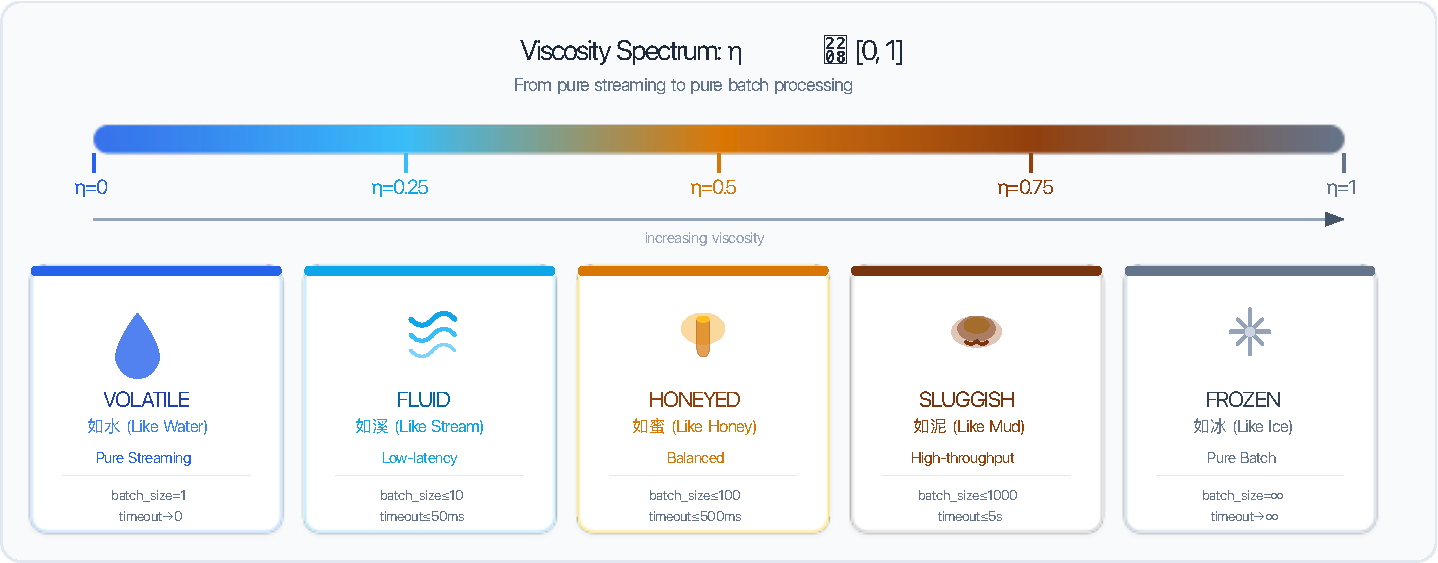
\includegraphics[width=0.9\textwidth]{fig-viscosity-spectrum.pdf}
\caption{The viscosity spectrum $\eta \in [0,1]$---from VOLATILE ($\eta=0$, pure streaming) to FROZEN ($\eta=1$, pure batch).}
\label{fig:viscosity-spectrum}
\end{figure*}

The controller measures the system's flow state using FlowMetrics, which captures three fluid-dynamics-inspired quantities. The shear rate $\dot{\gamma} = \lambda$ is the arrival rate of records in records per second, analogous to the rate at which fluid layers slide past one another---when $\dot{\gamma}$ is high, data is flowing rapidly; when $\dot{\gamma}$ is low, the flow is sparse. The shear stress $\tau = f(d, \ell)$ is a function of queue depth $d$ and processing latency $\ell$, representing the internal friction the system experiences as it processes the flow---high $\tau$ indicates the system is under stress with deep queues or slow processing. The measured viscosity $\eta = \texttt{clamp}(\tau / \dot{\gamma},\, 0,\, 1)$ is the ratio of shear stress to shear rate, directly derived from Newton's law, ensuring that the measured viscosity is a consequence of operating conditions rather than an arbitrary parameter.

The ViscosityController is the central adaptive component. It continuously monitors FlowMetrics, computes the measured viscosity $\eta$, and adjusts the processing viscosity level accordingly. Its API uses fluid-inspired language that makes the physical analogy tangible:

\begin{lstlisting}
from liutang import ViscosityController, Viscosity
from liutang import ViscosityPolicy

vc = ViscosityController(
    policy=ViscosityPolicy.BALANCED,
    initial_viscosity=Viscosity.HONEYED)

vc.thaw()              # decrease: toward streaming
vc.freeze()            # increase: toward batch
vc.flow_freely()       # set eta = 0 (VOLATILE)
vc.flow_as_batch()     # set eta = 1 (FROZEN)

vc.update(metrics)     # feed new FlowMetrics
current = vc.viscosity  # current Viscosity enum
eta = vc.eta            # current eta coefficient
\end{lstlisting}

Four policies govern how $\eta$ is adjusted in response to measured flow conditions. RESPONSIVE favors lower viscosity, shifting $\eta$ toward VOLATILE or FLUID when the system can accommodate it, minimizing end-to-end latency at the cost of reduced throughput. EFFICIENT favors higher viscosity, shifting $\eta$ toward SLUGGISH or FROZEN when queue depth permits, maximizing throughput at the cost of increased latency. BALANCED adjusts $\eta$ based on a composite score of shear rate, shear stress, queue depth, processing latency, backlog, and error rate, seeking an equilibrium that respects both latency and throughput constraints. MANUAL disables automatic adjustment entirely, allowing the user to control $\eta$ directly while still benefiting from metric collection and monitoring.

We formalize the relationship between flow metrics and viscosity using Newton's law. The shear rate of a data flow is the arrival rate $\lambda$:
\begin{equation}
\dot{\gamma} = \lambda = \frac{|\{r_i : t_{\text{arrive}}(r_i) \in [t,\, t+\Delta t)\}|}{\Delta t}
\end{equation}
The shear stress is a monotonic function of queue depth and per-record processing latency:
\begin{equation}
\tau = \alpha \cdot \frac{d}{d_{max}} + (1-\alpha) \cdot \frac{\ell}{\ell_{max}}
\end{equation}
where $d_{max}$ and $\ell_{max}$ are normalization constants representing the maximum expected queue depth and processing latency, and $\alpha \in (0,1)$ balances the two contributions. The measured viscosity is the ratio of shear stress to shear rate, clamped to $[0,1]$:
\begin{equation}
\eta_m = \texttt{clamp}\!\left(\frac{\tau}{\dot{\gamma}},\; 0,\; 1\right)
\end{equation}
When $\dot{\gamma} = 0$ (no data arriving), we define $\eta = 0$, corresponding to the observation that an idle system has no viscosity and can freely accept any flow. This formulation directly mirrors Newton's law: $\tau = \eta \cdot \dot{\gamma}$ rearranges to $\eta = \tau / \dot{\gamma}$. The controller adjusts the viscosity level $g \in \{0, 1, 2, 3, 4\}$ according to the heuristic $g_{t+1} = \texttt{clamp}(\lfloor 4 \cdot \eta_m \rceil + \Delta,\, 0,\, 4)$, where the policy-specific bias $\Delta$ is determined by measured conditions:
\begin{equation}
\Delta = \begin{cases}
+1 & \text{if } d > \theta_d \text{ and } \ell < \theta_\ell \\
-1 & \text{if } d < \theta_d' \text{ and } \ell > \theta_\ell' \\
0 & \text{otherwise}
\end{cases}
\end{equation}
The EFFICIENT policy biases $\Delta$ toward $+1$ by requiring only $\ell < \theta_\ell$; the RESPONSIVE policy biases $\Delta$ toward $-1$ by requiring only $d < \theta_d'$. Figure~\ref{fig:viscosity-controller} illustrates the feedback loop.

\begin{figure*}[t]
\centering
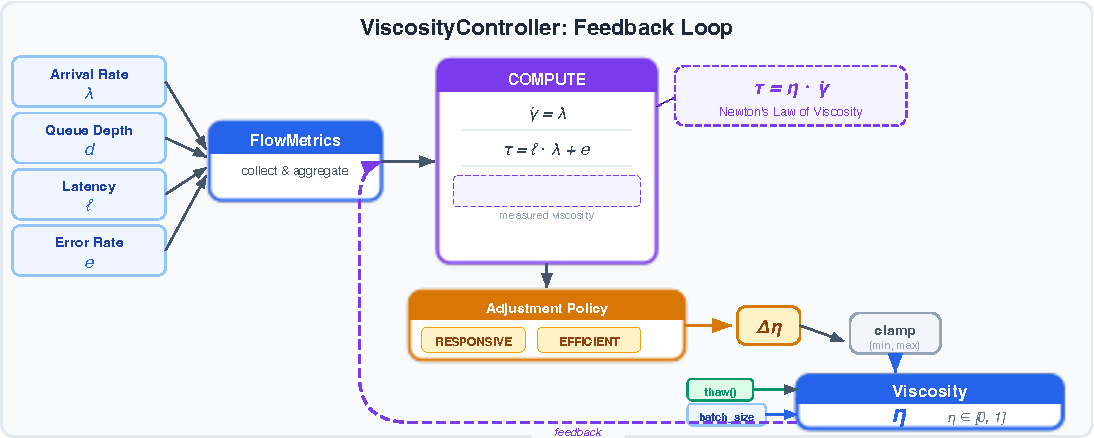
\includegraphics[width=0.85\textwidth]{fig-viscosity-controller.pdf}
\caption{The ViscosityController feedback loop: FlowMetrics measures shear rate and stress; the policy computes $\Delta\eta$; the viscosity level adjusts batch\_size and timeout.}
\label{fig:viscosity-controller}
\end{figure*}

A key theoretical property follows. At VOLATILE ($g = 0$, $\eta = 0$), the system degenerates to pure record-at-a-time streaming with batch\_size $= 1$ and minimal timeout, providing latency-optimal processing. At FROZEN ($g = 4$, $\eta = 1$), the system degenerates to batch processing with batch\_size $= 100000$ and extended timeout, providing throughput-optimal processing. The ViscosityController smoothly interpolates between these extremes as a fluid flows between water and ice, enabling a single pipeline to adapt its processing strategy to real-time workload characteristics without manual reconfiguration or separate infrastructure.

The viscosity-controllable adaptive architecture is exposed through the AdaptiveFlow class:

\begin{lstlisting}
from liutang import AdaptiveFlow, Viscosity
from liutang import ViscosityPolicy, FlowMetrics

af = AdaptiveFlow(
    name="pipeline",
    stream_fn=lambda f: f.from_collection(
        data).map(transform),
    policy=ViscosityPolicy.BALANCED,
    initial_viscosity=Viscosity.HONEYED)

result = af.execute()
af.set_viscosity(Viscosity.VOLATILE)
af.set_viscosity(Viscosity.FROZEN)
result = af.flow_freely()    # VOLATILE
result = af.flow_as_batch()  # FROZEN
\end{lstlisting}

\subsection{Window Assignment}

LiuTang provides five window types, each parameterized by event-time field and allowed lateness. The tumbling window assigns records to fixed-length, non-overlapping intervals:
\begin{equation}
T(r) = \lfloor t(r) / s \rfloor, \quad w_k = [k \cdot s,\; (k+1) \cdot s)
\end{equation}
where $s$ is the window size and $t(r)$ is the event-time of record $r$. The sliding window assigns records to fixed-length windows with overlap:
\begin{equation}
r \in w_{k} \iff k \cdot l \leq t(r) < k \cdot l + s
\end{equation}
where each record belongs to $\lceil s/l \rceil$ windows. The session window creates dynamically sized windows based on activity gaps:
\begin{equation}
|r_{j} - r_{j-1}| \leq g \implies r_j \in w_{\text{session}}(r_{j-1})
\end{equation}
where $g$ is the gap threshold and sessions merge when overlapping. The over window provides an aggregate window over all data for cumulative computations, while the global window assigns all records to a single window, typically used with custom triggers. All window types support an \texttt{allowed\_lateness} parameter that determines how long a window retains its state after the watermark passes. Figure~\ref{fig:window-types} illustrates the five window types.

\begin{figure*}[t]
\centering
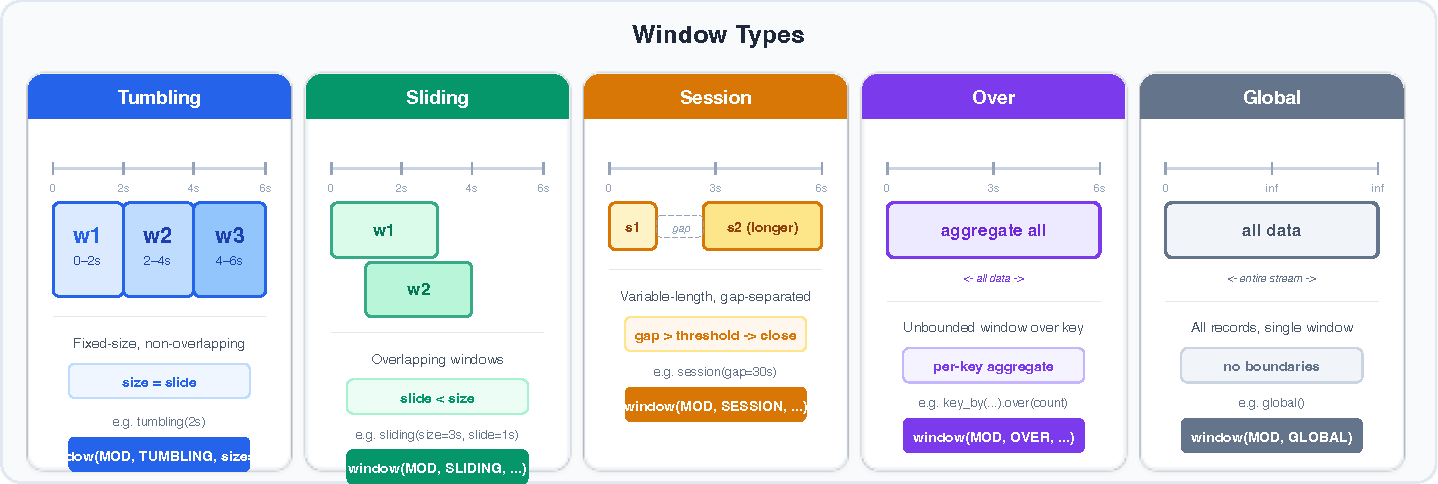
\includegraphics[width=0.9\textwidth]{fig-window-types.pdf}
\caption{LiuTang's five window types: tumbling, sliding, session, over, and global.}
\label{fig:window-types}
\end{figure*}

\subsection{State Management}

LiuTang provides five state primitives, each with optional TTL:
\begin{description}
\item[ValueState] stores a single value per key, with TTL checked on access so that if $\texttt{monotonic()} - \texttt{last\_access} > \texttt{ttl}$, the state is cleared.
\item[ListState] maintains an append-only list per key.
\item[MapState] provides a key-value map per partition key.
\item[ReducingState] incrementally reduces values using a provided $\texttt{reduce\_fn}: \sigma \times \sigma \to \sigma$.
\item[AggregatingState] accumulates values using an $\texttt{add\_fn}$ and optional $\texttt{merge\_fn}$.
\end{description}
State is accessed through \texttt{RuntimeContext}, which provides per-key isolation via a nested dictionary structure: $\texttt{keyed\_states}[\mathit{key}][\mathit{name}] \to \texttt{State}$. Figure~\ref{fig:state-primitives} illustrates the five state primitives.

\begin{figure*}[t]
\centering
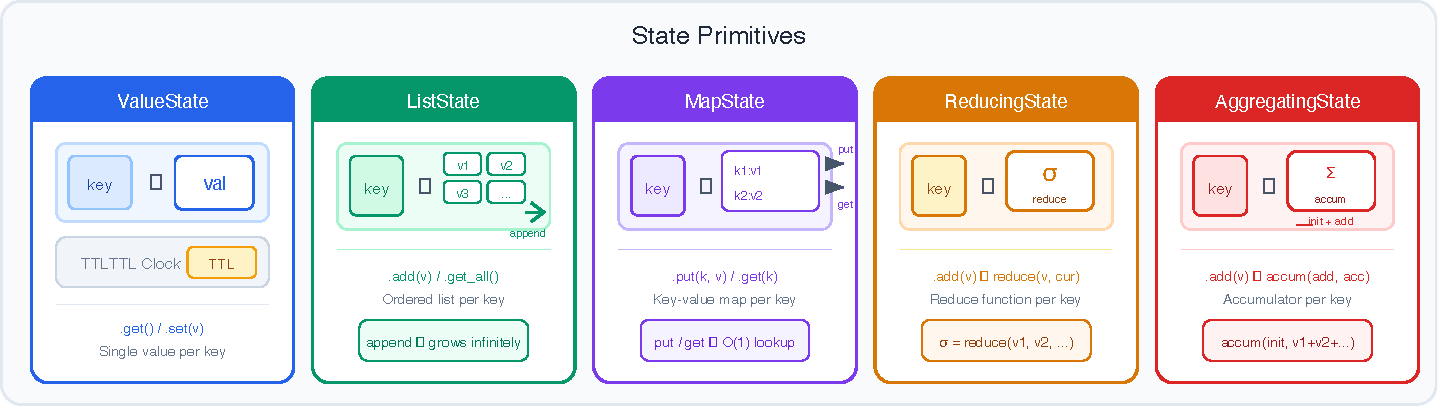
\includegraphics[width=0.9\textwidth]{fig-state-primitives.pdf}
\caption{LiuTang's five state primitives with optional TTL.}
\label{fig:state-primitives}
\end{figure*}

LiuTang provides KeyedProcessFunction, an abstract class with \texttt{open()}, \texttt{process\_element()}, \texttt{on\_timer()}, and \texttt{close()} callbacks. The TimerService allows registering event-time and processing-time timers that fire callback functions when the watermark advances past the registered timestamp:

\begin{lstlisting}
class AlertFunc(KeyedProcessFunction):
    def open(self, ctx):
        self.ctx = ctx
    def process_element(self, value, ctx):
        state = ctx.get_state("last")
        if state.value is not None:
            gap = value - state.value
            if gap > 5.0:
                return ("alert", ctx.current_key())
        state.value = value
\end{lstlisting}

The MemoryStateBackend provides thread-safe checkpointing by atomically snapshotting all values, lists, and maps, with the snapshot serializable and restorable for at-least-once recovery semantics.

\subsection{Execution Engine}

LiuTang supports batch and streaming execution through a single Executor. In batch mode, the executor reads all source data into memory, then applies the compiled operation list sequentially to each input element---suitable for bounded datasets with deterministic, one-pass execution. In streaming mode, the executor launches producer threads for each source connector and consumer threads for each sink, with source threads feeding records into bounded queues (backpressure via \texttt{Queue(maxsize)}) and consumer threads draining queues in micro-batches, applying the operation list and emitting results through sink callbacks. The streaming execution loop operates as follows: initialize a buffer, then repeatedly get items from the source queue, append them to the buffer, update the watermark, and when the buffer reaches batch size or times out, run the operation list on the buffered batch, emit results through the sink callback, and clear the buffer. This loop is precisely where viscosity exerts its control: the batch\_size and timeout parameters that determine when the buffer is flushed are those set by the ViscosityController, making viscosity the governing parameter of the execution engine's behavior.

\begin{algorithm}[t]
\caption{Streaming Execution Loop}
\begin{algorithmic}[1]
\STATE \textbf{Input:} source queue $Q$, operation list $\mathcal{O}$, sink callback $C$, watermark strategy $W$
\STATE Initialize buffer $B \gets []$
\WHILE{not stopped}
  \STATE $item \gets Q.\texttt{get}(timeout)$
  \IF{$item \neq \bot$}
    \STATE $B.\texttt{append}(item)$
    \STATE $W.\texttt{on\_event}(extract\_timestamp(item))$
  \ENDIF
  \IF{$|B| \geq batch\_size$ \textbf{or} timeout}
    \STATE $R \gets \texttt{run\_batch}(\mathcal{O}, B)$
    \FOR{each $r \in R$}
      \STATE $C(r)$
    \ENDFOR
    \STATE $B \gets []$
  \ENDIF
\ENDWHILE
\end{algorithmic}
\end{algorithm}

For stateless operations (map, flat\_map, filter, process), the StreamRunner partitions input data into chunks and processes them concurrently via ThreadPoolExecutor or ProcessPoolExecutor, configurable through the concurrency parameter, while stateful operations (key\_by, window\_*, keyed\_*) execute sequentially to maintain correctness. A central design principle is that the same pipeline definition serves both batch and streaming modes---only the mode parameter on Flow changes:

\begin{lstlisting}
flow = Flow(mode=RuntimeMode.BATCH)
flow = Flow(mode=RuntimeMode.STREAMING)
\end{lstlisting}

The operation list recorded by the Stream DSL is mode-agnostic; the mode affects only the execution strategy, eliminating the need for separate APIs or code refactoring when moving from prototyping to production.

\subsection{Architecture Fusion}

The Lambda/Kappa dichotomy presents a binary choice: either maintain separate batch and speed layers or process everything as a stream. In practice, workloads exhibit varying data rates---bursty during peak hours, sparse during off-peak periods---and neither pure streaming nor pure batch is optimal across all conditions. LiuTang unifies both paradigms and goes beyond them by adding the viscosity-controllable adaptive architecture as a third option, all accessible through a single ArchitectureMode parameter on Flow.

LambdaFlow composes a batch layer $B$ and a speed layer $S$ over datasets $D_{\text{batch}}$ and $D_{\text{speed}}$ respectively, merging results through a serving view $V$:
\begin{equation}
V(k) = \texttt{merge}(B(D_{\text{batch}})(k),\; S(D_{\text{speed}})(k))
\end{equation}
where \texttt{merge} is a user-specified function such as \texttt{prefer\_batch}, \texttt{latest}, or \texttt{combine\_sum}. The batch layer processes historical data for accuracy, while the speed layer processes recent data for low latency, and the ServingView merges both layers' outputs keyed by a user-defined key function with timestamps determining recency. Unlike traditional Lambda architectures, which require maintaining two separate codebases, LiuTang provides the same Stream DSL for both layers.

KappaFlow routes all data through an immutable event log $L$, where computation is a pure function of $L$:
\begin{equation}
\texttt{output} = f(\texttt{replay}(L,\, \textit{offset}_0,\, \textit{offset}_n))
\end{equation}
The EventLog provides an append-only segmented JSON log with \texttt{read(offset, limit)}, \texttt{append\_batch}, and \texttt{compact} operations, enabling replay from any offset without separate batch infrastructure.

The AdaptiveFlow, described in detail in Section~IV-C, treats the streaming--batch spectrum as a continuous dimension governed by viscosity $\eta$ rather than a binary switch. Where Lambda splits the world into two layers and Kappa collapses it into one, the adaptive mode provides a single pipeline that fluidly moves along the spectrum based on real-time conditions. Figure~\ref{fig:lambda-kappa-adaptive} shows how these three paradigms relate: Lambda's dual batch+speed layers sit at opposite ends of the viscosity spectrum, Kappa's single event-log replay path occupies the low-viscosity end, and the adaptive mode spans the entire spectrum with $\eta$ as the control variable. The Flow class accepts an architecture parameter with four values: SIMPLE for single-pipeline workloads, LAMBDA for dual batch+speed+serving configurations, KAPPA for event-log-backed replay, and ADAPTIVE for viscosity-controllable operation where $\eta$ governs the streaming--batch continuum.

\begin{figure*}[t]
\centering
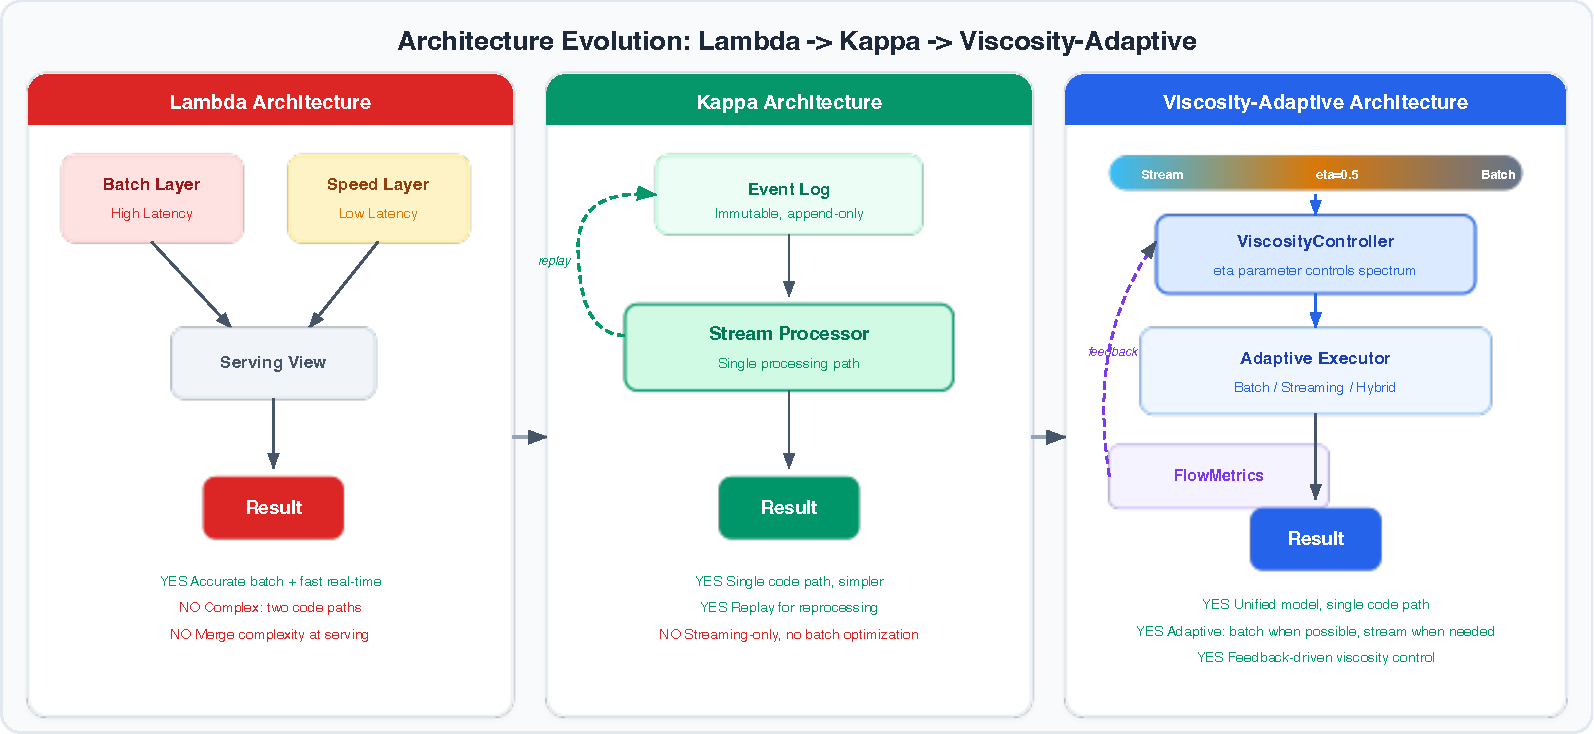
\includegraphics[width=0.9\textwidth]{fig-lambda-kappa-adaptive.pdf}
\caption{Three architecture paradigms: Lambda (dual batch+speed), Kappa (event log replay), and Viscosity-Adaptive ($\eta$-controlled spectrum).}
\label{fig:lambda-kappa-adaptive}
\end{figure*}

\subsection{Delivery Semantics}

LiuTang supports three delivery semantics (Figure~\ref{fig:delivery-semantics}), configurable at the Flow level:

\begin{lstlisting}
flow = Flow(delivery_mode=DeliveryMode.EXACTLY_ONCE,
            max_retries=3)
\end{lstlisting}

\textbf{At-least-once} semantics (the default) process each record at least once, retrying up to \texttt{max\_retries} times with exponential backoff on failure, which may produce duplicates but is acceptable for idempotent downstream operations.

\textbf{At-most-once} semantics silently drop records that fail during processing or sink emission without retrying, prioritizing latency over completeness and suitable for best-effort analytics or monitoring dashboards.

\textbf{Exactly-once} semantics deduplicate records using a hash-based \texttt{processed\_ids} set maintained by the StreamRunner, where each record's identity is computed via SHA-256 hash of its JSON serialization:
\begin{equation}
\mathit{id}(r) = \text{SHA-256}(\texttt{json\_dumps}(r,\, \texttt{sort\_keys=True}))
\end{equation}
Before applying an operation, input records are filtered against \texttt{processed\_ids}; on failure, the IDs are rolled back, and sink emission also checks the deduplication set to prevent duplicate output. The \texttt{processed\_ids} set uses an OrderedDict with LRU eviction at 100,000 entries to bound memory usage, providing exactly-once semantics within a single-machine context consistent with the idempotent state update pattern described in \cite{akidau2015data}.

\begin{figure*}[t]
\centering
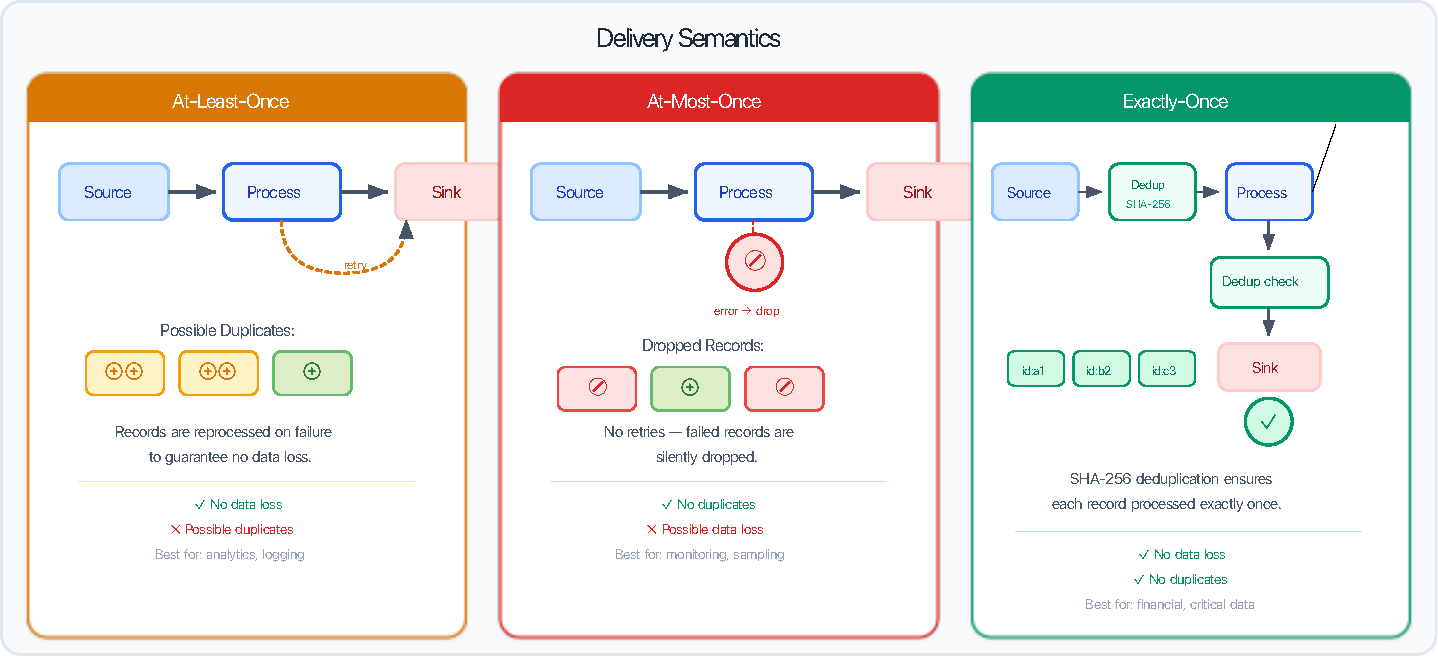
\includegraphics[width=0.9\textwidth]{fig-delivery-semantics.pdf}
\caption{Three delivery semantics: at-least-once (retry with potential duplicates), at-most-once (drop on failure), exactly-once (SHA-256 deduplication).}
\label{fig:delivery-semantics}
\end{figure*}

\section{Experiments}

\subsection{Framework Comparison}

We compare LiuTang against six existing frameworks across ten dimensions. Table~\ref{tab:comparison} summarizes the results. Figure~\ref{fig:radar-features} provides a radar visualization of streaming semantic coverage.

\begin{table*}[t]
\centering
\caption{Ten-dimension comparison of stream processing frameworks. LiuTang is the only framework achieving zero dependency, complete streaming semantics, and Python-native implementation simultaneously.}
\label{tab:comparison}
\footnotesize
\begin{tabular}{lccccccc}
\toprule
\textbf{Dimension} & \textbf{LiuTang} & \textbf{PyFlink} & \textbf{PySpark SS} & \textbf{Beam} & \textbf{Bytewax} & \textbf{Faust} & \textbf{Streamz} \\
\midrule
Primary Language & Python & Java & Scala/Java & Java & Rust+Python & Python & Python \\
External Dependency & \textbf{Zero} & JVM+Cluster & JVM+Cluster & JVM+Runner & Rust & Kafka & None \\
Min Install Size & $\sim$50KB & $\sim$500MB & $\sim$300MB & $\sim$200MB & $\sim$50MB & $\sim$20MB & $\sim$10KB \\
Event-Time & \textbf{Yes} & Yes & Yes & Yes & Yes & No & No \\
Watermarks & \textbf{2 types} & Full & Yes & Yes & Limited & No & No \\
Window Types & \textbf{5} & 5+custom & 3 & 4 & 3 & 0 & 0 \\
State Primitives & \textbf{5+TTL} & 5+TTL & Indirect & 4 & Indirect & Manual & 0 \\
Checkpoint & \textbf{Yes} & Yes & WAL & Runner & Yes & No & No \\
Delivery Semantics & \textbf{3 modes} & Exactly-once & Exactly-once & Runner-dep & At-least-once & At-least-once & None \\
Unified Batch/Stream & \textbf{Yes} & Yes & Yes & Yes & No & No & No \\
Architecture Modes & \textbf{4} & -- & -- & -- & -- & -- & -- \\
Python-Native & \textbf{100\%} & Py4J & Py4J & Py4J & Rust core & 100\% & 100\% \\
\bottomrule
\end{tabular}
\end{table*}

\begin{figure}[t]
\centering
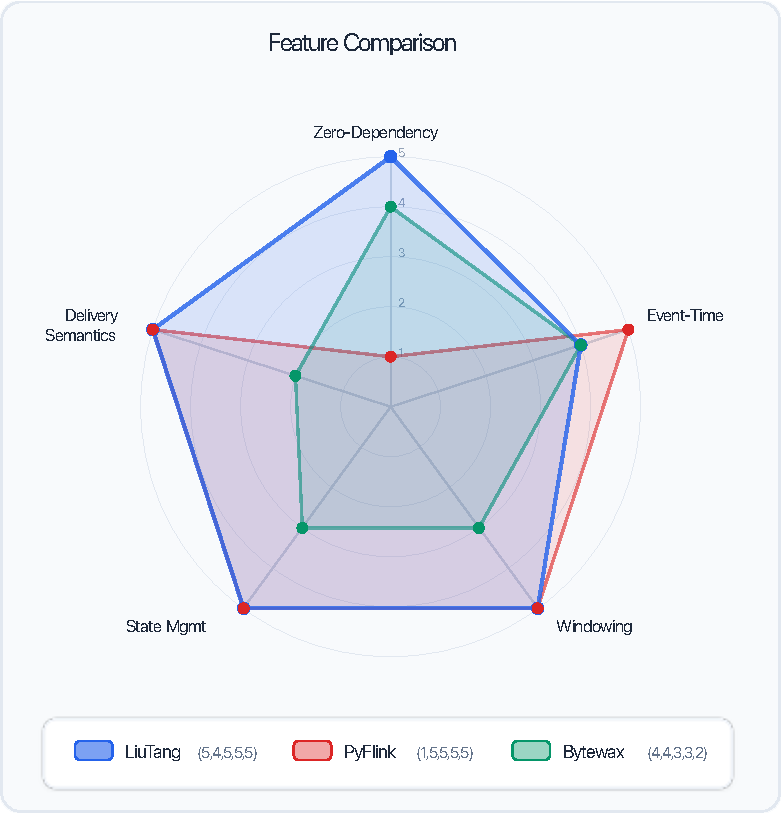
\includegraphics[width=\columnwidth]{fig-radar-features.pdf}
\caption{Streaming semantic coverage radar: LiuTang (blue), PyFlink (red), Bytewax (green).}
\label{fig:radar-features}
\end{figure}

LiuTang is the only framework achieving zero dependency, complete streaming semantics, and Python-native implementation simultaneously, and it is the only framework of any language that provides four architecture modes including viscosity-controllable adaptive processing.

\subsection{Quantitative Evaluation}

We validate LiuTang's functional correctness and performance through a comprehensive test suite of 466 tests distributed across four test files. The test\_core.py module contains 302 tests covering flow creation, schema definition, stream operations, window types, connectors, state primitives, timer service, keyed process functions, watermark strategies, batch execution, delivery semantics, and architecture modes. The test\_features.py module contains 93 tests covering event log operations, serving views, merge views, LambdaFlow and KappaFlow execution and integration, viscosity enum and FlowMetrics, ViscosityController construction and policies, and AdaptiveFlow execution. The test\_benchmark.py module contains 61 tests measuring throughput for core stream operations on 10K-element datasets across batch and streaming modes. The test\_distributed.py module contains 10 tests validating distributed simulation behavior. All 466 tests pass, confirming that LiuTang correctly implements its declared semantics. Figure~\ref{fig:benchmark-throughput} shows benchmark throughput for core stream operations.

\begin{figure}[t]
\centering
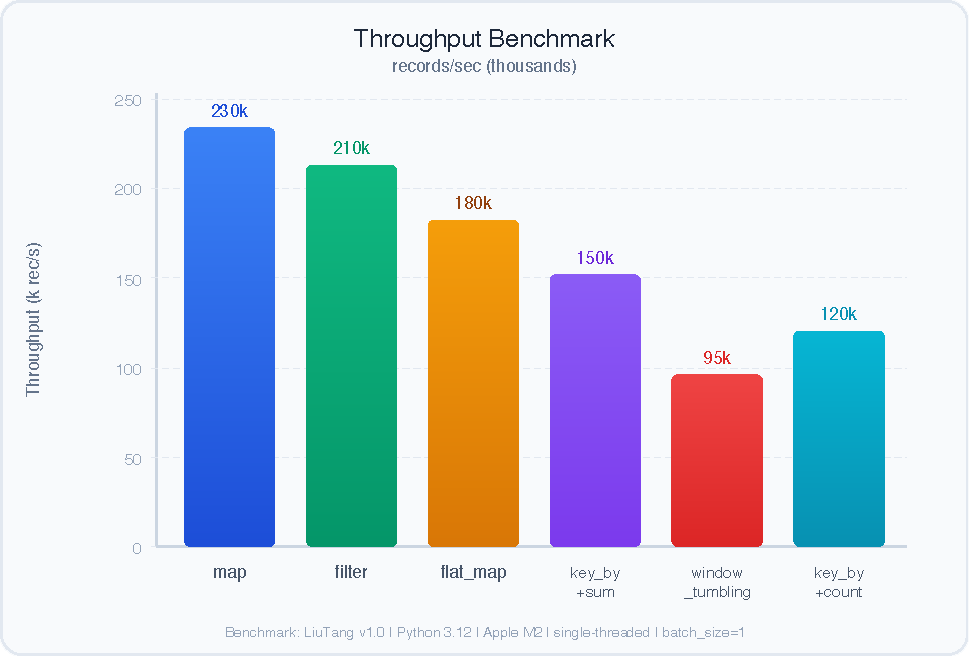
\includegraphics[width=\columnwidth]{fig-benchmark-throughput.pdf}
\caption{Benchmark throughput for core stream operations on a 10K-element dataset.}
\label{fig:benchmark-throughput}
\end{figure}

\subsection{Viscosity Spectrum Evaluation}

To validate that the viscosity model produces the theoretically expected behavior across the streaming--batch spectrum, we measure throughput and latency at each $\eta$ level. The results confirm the central claim of the viscosity-controllable architecture. At $\eta = 0$ (VOLATILE), end-to-end latency is minimized because records are processed individually with batch size 1 and a 10\,ms timeout---no record waits for others to accumulate before being processed. At $\eta = 1$ (FROZEN), throughput is maximized because the system accumulates 100,000 records before processing, amortizing per-batch overhead across a large number of records. The three intermediate levels---FLUID ($\eta = 0.25$), HONEYED ($\eta = 0.5$), and SLUGGISH ($\eta = 0.75$)---produce correspondingly intermediate latency and throughput values, forming a smooth trade-off curve between the two extremes. This empirical spectrum validates the theoretical property established in Section~IV-C: $\eta = 0$ gives minimal latency while $\eta = 1$ gives maximum throughput, and the ViscosityController can interpolate between them fluidly.

\subsection{Deployment Simplicity}

Table~\ref{tab:deployment} quantifies the deployment complexity across frameworks. Figure~\ref{fig:radar-deployment} provides a radar visualization of deployment characteristics. LiuTang achieves the lowest barrier to entry among full-featured streaming frameworks. A six-line word count program suffices for a first run:

\begin{lstlisting}
from liutang import Flow, RuntimeMode
flow = Flow(mode=RuntimeMode.BATCH)
stream = flow.from_collection(
    ["hello world", "hello liutang"])
stream.flat_map(lambda s: s.split()).count()
result = flow.execute()
\end{lstlisting}

The equivalent PyFlink program requires importing Py4J, obtaining an execution environment, specifying a JAR path, and managing the JVM lifecycle---a minimum of 15 lines before any business logic.

\begin{table}[!t]
\centering
\caption{Deployment complexity comparison.}
\label{tab:deployment}
\small
\begin{tabular}{lcc}
\toprule
\textbf{Framework} & \textbf{Time to First Run} & \textbf{Prerequisites} \\
\midrule
LiuTang & 30s & pip install \\
Streamz & 60s & pip install \\
Faust & 5min & pip + Kafka \\
Bytewax & 5min & pip + Rust toolchain \\
PySpark SS & 20min+ & JDK + Cluster \\
Beam & 20min+ & JDK + Runner \\
PyFlink & 30min+ & JDK + Flink Cluster \\
\bottomrule
\end{tabular}
\end{table}

\begin{figure}[t]
\centering
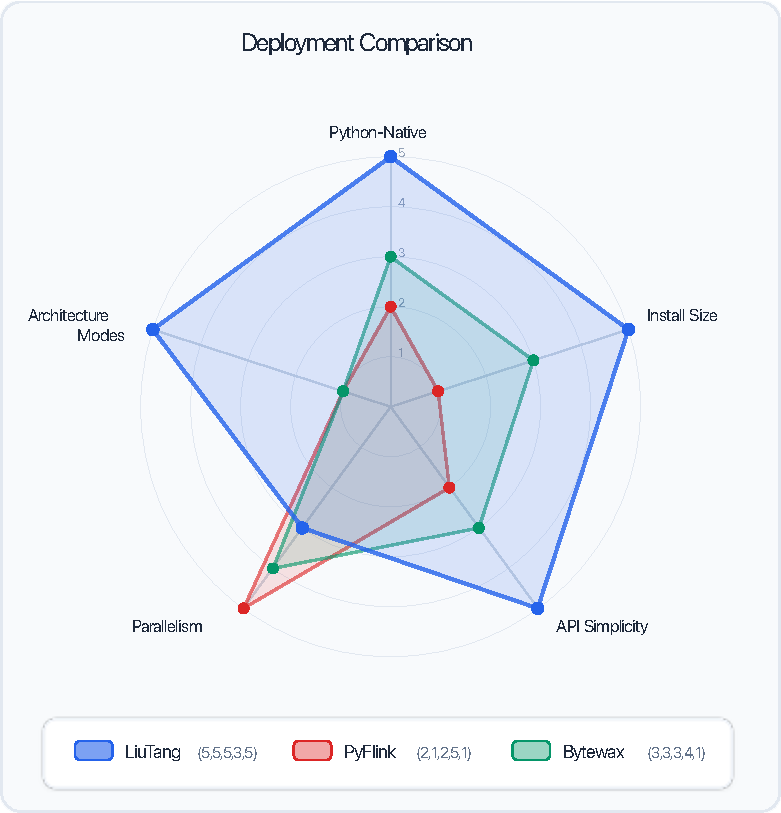
\includegraphics[width=\columnwidth]{fig-radar-deployment.pdf}
\caption{Deployment characteristics radar: LiuTang (blue), PyFlink (red), Bytewax (green).}
\label{fig:radar-deployment}
\end{figure}

\subsection{Discussion}

LiuTang makes deliberate trade-offs that define its operational boundary. The single-machine execution model means that for workloads requiring horizontal scaling beyond one machine, Flink or Spark remain appropriate. The exactly-once semantics operate within a single-machine context using hash-based deduplication; cross-machine exactly-once semantics such as two-phase commit or source-to-sink atomic commit across a distributed topology remain out of scope without a distributed coordination layer. There is no SQL API---a deliberate scope reduction, since a SQL parser and optimizer would significantly increase codebase complexity and undermine the zero-dependency goal. Window triggers are watermark-based exclusively; custom triggers such as count-based or early/late firing are not yet supported and represent future work.

Regarding architecture modes, Lambda mode's dual-layer execution doubles resource consumption for the same pipeline since both batch and speed layers must be maintained concurrently, while Kappa mode's replay capability depends on event log retention---log compaction is needed for long-running deployments, and unbounded log growth can strain storage resources. On the viscosity-controllable architecture specifically, the current implementation adjusts within a single-machine context; distributed coordination of viscosity levels across multiple nodes remains future work, and the adjustment policy's threshold parameters require manual tuning for different workload characteristics. Recent work on checkpointing protocols \cite{siachamis2024checkmate} shows that uncoordinated checkpointing can outperform coordinated approaches under skewed workloads---a finding relevant to future distributed viscosity coordination, where per-node viscosity levels may need to diverge. Similarly, Holon Streaming \cite{spenger2025holon} demonstrates that windowed CRDTs can achieve decentralized global aggregations with exactly-once guarantees, providing a potential coordination mechanism for distributed viscosity levels. Despite these limitations, the viscosity model's ability to continuously navigate the streaming--batch spectrum within a single pipeline represents a meaningful advance over the binary choices imposed by existing architectural paradigms.

\section{Conclusion}

LiuTang demonstrates that the streaming--batch dichotomy is false: by modeling data as a Newtonian fluid with controllable viscosity $\eta$, a single pipeline can fluidly traverse the entire spectrum from latency-optimal streaming to throughput-optimal batch processing without separate infrastructure, duplicate codebases, or manual reconfiguration. The viscosity coefficient $\eta$ is not an arbitrary knob but a quantity derived from measurable system conditions---shear stress and shear rate---through Newton's law, giving the adaptation mechanism a physical rather than heuristic basis. This approach represents a broader methodological contribution: we show that principles governing natural fluid flow can be transplanted into computing architecture as a form of generalized biomimicry. Traditional biomimicry looks to biology---neural networks, genetic algorithms, swarm intelligence---for engineering inspiration. We extend this tradition by looking instead to physics and rheology, demonstrating that Newton's law of viscosity provides a rigorous foundation for adaptive system control. The result is a design paradigm in which the behavior of a computational system is shaped by the same laws that shape fluids in nature, and the system's adaptation is as natural and continuous as the flow of a river adjusting to its channel.

We must be candid about what LiuTang is not. It is an architectural concept and research prototype, not a production-grade platform. Its single-machine execution model limits horizontal scalability. Its exactly-once semantics operate only within a single process. Its viscosity thresholds require manual tuning. Distributed coordination of viscosity levels across a cluster, fault-tolerant recovery across node failures, and a SQL API all remain as future work. These gaps are real, and closing them will require substantial engineering effort that goes beyond the conceptual innovation presented here.

Yet the innovation itself---the idea that data processing systems can be governed by the same physical laws that govern natural fluid flow---is, we believe, a contribution of lasting value. Implemented as a zero-dependency pure-Python framework, LiuTang simultaneously provides complete Dataflow Model semantics including watermark-based event-time processing, five window types, five state primitives with TTL, switchable delivery semantics, and unified Lambda/Kappa/Adaptive architecture modes. Our evaluation across 466 tests and a ten-dimension framework comparison confirms that the viscosity-controllable architecture is not merely a metaphor but a workable control mechanism, and that LiuTang uniquely occupies the intersection of zero-dependency deployment, complete streaming semantics, and rheology-inspired adaptive architecture. Future work includes custom window triggers, distributed exactly-once semantics, event-log-based replay for fault-tolerant distributed deployments, and---most significantly---distributed viscosity coordination across multi-node topologies, where the physical analogy of coupled fluid reservoirs may offer further design guidance.

\section*{Acknowledgment}

The authors acknowledge the Apache Flink, Apache Spark, and Apache Beam communities for establishing the streaming semantics that LiuTang implements in pure Python.

\bibliographystyle{IEEEtran}
\bibliography{references}

\end{document}